
%\documentclass[reprint,amsmath,amssymb, aps, twocolumn,]{revtex4-1}
\documentclass[reprint,amsmath,amssymb, aps, 10pt, a4paper, english, reqno]{revtex4-1}


\newcommand{\dd}{\textrm{d}}
\usepackage{braket}
\usepackage{lipsum, babel}
\usepackage{blindtext}
\usepackage{graphicx}% Include figure files
\usepackage{dcolumn}% Align table columns on decimal point
\usepackage{bm}% bold math
\usepackage{listings}
\usepackage{listing}
\usepackage{supertabular}



\usepackage{color} %red, green, blue, yellow, cyan, magenta, black, white
\definecolor{mygreen}{RGB}{28,172,0} % color values Red, Green, Blue
\definecolor{mylilas}{RGB}{170,55,241}



\lstset{language=Matlab,%
    %basicstyle=\color{red},
    breaklines=true,%
    morekeywords={matlab2tikz},
    keywordstyle=\color{blue},%
    morekeywords=[2]{1}, keywordstyle=[2]{\color{black}},
    identifierstyle=\color{black},%
    stringstyle=\color{mylilas},
    commentstyle=\color{mygreen},%
    showstringspaces=false,%without this there will be a symbol in the places where there is a space
    numbers=left,%
    numberstyle={\tiny \color{black}},% size of the numbers
    numbersep=9pt, % this defines how far the numbers are from the text
    emph=[1]{for,end,break},emphstyle=[1]\color{red}, %some words to emphasise
    %emph=[2]{word1,word2}, emphstyle=[2]{style},    
}



\begin{document}

%\preprint{APS/123-QED}

\title{Lennard-Jones Potential Simulation.}% Force line breaks with \\
\thanks{Analysis based on Computational Physics module.}%

\author{Timothy Holmes}
 \altaffiliation{Department of Physics and Astrophysics, DePaul University, IL}%Lines break automatically or can be forced with \\

DePaul University, Chicago, IL\\

\date{\today}% It is always \today, today,
             %  but any date may be explicitly specified
\setlength\parindent{0pt}
\begin{abstract}

\setlength\parindent{0pt}
The Lennard-Jones potential is an equation that helps determine the potential energy of a molecular system. This potential can also be used to simulate the forces of molecules. This computational experiment implements a basic molecular dynamics program to simulate a gas molecule system in 2 dimensions and 3 dimensions. This experiment was ran with two different numerical methods, the Euler's integration method and  the velocity Verlet method. Comparing these two methods, Euler's method would result in a chaotic system immediately when boundary conditions were imposed. While the Verlet method would also fail, the system would stay stable for some time based on initial conditions. A system without boundary conditions would never become unstable since not molecules in the system would have unstable velocities. Changing values $\sigma$ and $\epsilon$ to an appropriate amount where both forces are not too powerful or weak was found to stabilize the program. 

\vspace{4mm}

\textit{Subject headings}: Molecular Dynamics --- Physics Simulation --- Lennard-Jones Potential

\end{abstract}

\pacs{Valid PACS appear here}% PACS, the Physics and Astronomy
                             % Classification Scheme.
%\keywords{Suggested keywords}%Use showkeys class option if keyword
                              %display desired
\maketitle

%\tableofcontents

\begin{multicols}{2}
\section{\label{sec:level1}Introduction}


The Lennard-Jones potential describes the potential energy interaction on atoms and molecules that are not bonded. The potential energy is calculated off the distance of each atoms or molecule in the system. Therefore, each atom interaction has an attractive force on one another as well as a repulsive force on one another. The interactions can be determined by the following scenarios. First, a system with just two atoms that an infinite distance apart will have no interaction, neither atom will want to attract or repeal each other. Say that these two atoms are now a distance of $r$ away from each other. The attractive force will bring these two atoms closer and closer together. This interaction will occur until a certain equilibrium distance is meet. At a certain point in the interaction the atoms will start to experience the repulsive force that will drive these atoms apart. It should be noted that in this scenario the repulsive fore is much greater than the attractive force. This qualitative scenario can be described quantitatively using the Lennard-Jones Potential. The Lennard-Jones Potential is given by the following equation, 

\begin{equation}
    V(r_{ij}) = \epsilon\Bigg[\Bigg(\frac{\sigma}{r_{ij}}\Bigg)^{12} - \Bigg(\frac{\sigma}{r_{ij}}\Bigg)^{6}\Bigg]
\end{equation}

where $V$ is the potential energy of the interaction, $\epsilon$ is the well depth and a measure of the attraction force, $\sigma$ is when the potential of two atoms is zeros which also indicates how close the particles can get before the repulsive force starts, and $r_{ij} = r_{i} - r_{j}$ is the distance of separation between both particles. Figure 1 below shows an example of the Lennard-Jones potential. 



\begin{center}
    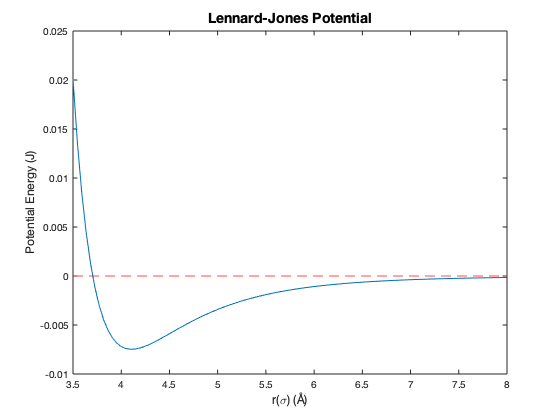
\includegraphics[width=0.50\textwidth]{lennard_jones_potential.png}
    \caption{\small FIG 1: The Lennard-Jones potential describes the attraction and repulsion of non bonding particles. To the left of the minimum of the well illustrates the repulsive force. To the right of the minimum of the well illustrates the attractive force.}
\end{center}

In Figure 1, the width between the y-axis and the blue line represent $\sigma$. This width will describe how close two  molecules can get before they repel each other. Furthermore, the height between the dotted red and the minimum of the well describes how strong the interaction is between two particles. Therefore, the larger $\sigma$ becomes the the distance between molecules will increases, that is, the range of the repulsive force increases. Likewise, the larger $\epsilon$ get the deeper the well will become and the it will increase the strength of attraction between two particles. \\

The repulsive force of equation (1) is the part with the power of 12 such that

\begin{equation}
E_{PE}(repulsive) = \Bigg(\frac{\sigma}{r_{ij}}\Bigg)^{12} 
\end{equation}

while the attractive force is the part of equation (1) with the power of 6 given by

\begin{equation}
E_{PE}(attraction) = - \Bigg(\frac{\sigma}{r_{ij}}\Bigg)^{6}.
\end{equation}

The combined sum of these two potential energies will give the total potential energy of the system. Given a scenario where two molecules are moving towards each other, the repulsive force occurs when the electron clouds of two molecules are close enough to repulsive force to repel these molecules. \\

When the forces are equal, the two molecules are at their equilibrium separation, both forces are zero. The attractive forces on two molecules will have negative potential energy on the system as a whole while the repulsive forces will have a positive potential energy on the system. The molecules in the system will always be wanting to move to where potential energy is zero. In equation (3), the repulsive force is inversely proportional to $r_{ij}^{6}$ which has a rapid decrease as two molecules move apart. In equation (2), the attractive forces inversely proportional to $r_{ij}^{12}$ which has a more rapid decrease than the repulsive force as two molecules move away from each other. This balance of forces can been seen again in Figure 1. A more detailed calculation of forces is described in section 2D.

%\clearpage

\section{Molecular Dynamics 2D System Simulation}

%\subsection{Initializing the System}

\subsection{Initializing Position}

The first step in setting up the simulations to to initialize all of the variables in the system. To start, the atoms in the system need to have some initial start position at $x0$, $y0$, and $z0$ for the 3D case. For the sake of simplicity this simulation will be ran using just the 2D case. There are a few ways to determine the initial position and depending on the type of material the positions ordering may matter. For a solid a crystalline lattice structure is an important property that solids have, where the pattern of the atoms matter. This attribute isn't true for liquids and gasses. For a liquid or a gas, the initial positions can be randomly generated with a symmetric $n \times n$ or an asymmetric $n \times m$ box. For observational purposes, the initial positions for all simulations are set up to have $n$ rows of atoms by $n$ columns of atoms that are spaced out by some length $L$. 

\subsection{Initializing Velocity}

The initial velocity also will depend on the material. It should be expected the velocity in a solid would be zero. Instead the atoms jiggle or vibrate. The hotter the material gets the faster these atoms will vibrate up to a point where the atoms have enough energy to break their bonds. At this point the solid matter would have a phase transition to a liquid where the velocity would now be relevant to the system. In gasses, more so ideal gasses such as argon, the atoms in this system will have an initial velocity and would be expected to be moving fast. The velocity of a given molecule in a system can be found by

\begin{equation}
    v_{p} = \sqrt{\frac{2*k*T}{m}}
\end{equation}

where $k$ is Bolzmann's constant, $T$ is temperature, and $m$ is the mass of the particle. This equation will give the velocity of a gas particle. Given the temperature of a gas as well as the molecular weight this equation can determine the velocity of a specific gas. The hotter the gas molecule and the lighter the molecule weighs, the faster it will travel. The cooler and heavier molecule, the slower it will travel. To better see the force interaction of simulation, a slower gas is preferred. \\

To test a system that is not based on real world numbers, velocity can also be randomly generated number that is unit-less. To Implement this strategy into the behaviour into the model, the rest of the model will also have to use unit-less variables. For example, just setting $m = 1$ to satisfy the acceleration calculation.  

\subsection{Boundary Conditions}

One final system set up includes boundary conditions. Within the $n \times n$ box contains all of the particles at $t = 0$, but this doesn't have to be the case as time increases. The program can allow for the systems particles to do one of two things. It can allow for the particles to travel to infinity in all spacial directions or it can contain the particles within a defines $n \times n$ box. The easiest to implement is the former boundary condition since it requires nothing additional to allow the particles to travel freely. Boundary conditions are useful when testing a system. A system without boundary conditions can tell you how certain molecules or a physical state will act when no other forces are acting on it. While a system with boundary conditions can explain the energy results, like a gas, in an enclosed confined space.

\subsection{Force Calculation}

One of the most critical calculations to get right in this simulation is the force calculation. Without the attractive force and the repulsive force, this simulation is simply just vectors on a graph. The points will have some initial velocity and direction with no interactions. This would defeat the purpose of this model as it would not actually model any physical phenomenon, it would simply model some random math problem. Calculating forces using numerical techniques is possible, however, this is often slow and analytically solving first and evaluating later will greatly speed up the model. If we wanted to find the force from atom $a$ acting on atom $b$ in the $x$ direction, the following derivative will solve for this problem,

\begin{equation}
\frac{\partial V(r_{ij})}{\partial x_{i}} = \frac{\partial V(r_{ij})}{\partial r_{ij}} \frac{\partial r_{ij}}{\partial x_{i}}
\end{equation}

where

\begin{equation}
f_{ij} = \frac{\partial V(r_{ij})}{\partial r_{ij}} \times \frac{r_{ij}}{r{ij}}
\end{equation}.

This is obviously for the 2D case, however, for the 3D case an extra $z$ 
component will be added on. Evaluating the partial derivatives above gives

\begin{equation}
\partial \frac{V(r_{ij})}{\partial x_{i}} 
\end{equation}

More generally the force can be wrote for all coordinates as

\begin{equation}
f_{r_{ij}} = \frac{24\epsilon}{r^{2}_{ij}}\Bigg[2\Bigg(\frac{\sigma}{r_{ij}}\Bigg)^{12} - \Bigg(\frac{\sigma}{r_{ij}}\Bigg)^{6}\Bigg]
\end{equation}

The final equation can then be implemented into the simulation to calculate force in each coordinate direction. \\

To avoid forces from extremely long distances, a cut off value needs to be implemented. A particles forces should only act on other particles if they are in a reasonable range. This is the forces should not have an affect if $r_{ij} > r_{c}$, however, the forces should remain in affect if $r_{ij} \le r_{c}$. This should have a smoothing affect that will prevent simulation errors as time increases. One problem that arises from this cut off value is energy calculations and the force calculations, that may spawn discontinuities that would have not originally occurred.

\subsection{Euler's Method}

There are many numerical methods to solve molecular dynamic systems. One of the most straight forward methods is to use the Euler's method. Euler's numerical integration method can be computed by the following

\begin{align}
    r(t + h) = r(t) + v(t)*h \\
    v(t + h) = v(t) + a(t)    
\end{align}


where $r$ is the distance from one atom to another, $t$ is time, $h$ is a time step, $v$ is velocity, and $a$ is acceleration. The acceleration is found by calculating the force $f$ and dividing by the mass $m$, such that $a = f/m$. This numerical method is a first order method. This method should not be used since there are better methods available that are just as easy to implement. 

\subsection{Velocity Verlet Method}

A better method in molecular dynamic simulations is to use the velocity Verlet numerical method. The Verlet numerical method is given by 

\begin{align}
    r(t + h) = r(t) + v(t)*h + a(t)*h^{2}\\
    v(t + h) = v(t) + a(t)
\end{align}

where $r$ is the distance from one atom to another, $t$ is time, $h$ is a time step, $v$ is velocity, and $a$ is acceleration. The idea behind this numerical method can be explained in a few simple steps, steps that help make it better than Euler's method. Each integration cycle of the Verlet algorithms starts with calculating the velocities at the mid-point step. From there the new positions are calculated. Then the accelerations are calculated from the potential. Finally, the velocities are updated. The Verlet method is a second order method. 
    

\section{\label{sec:level3}DISCUSSION} 

\subsection{Molecular Dynamics 2D System Discussion}

There are many things that this simulation can tell about the system. This simulation will produce data that will estimate the changes is kinetic energy, potential energy, total energy, temperature, pressure, attractive force, and the repulsive force. \\

\begin{center}
    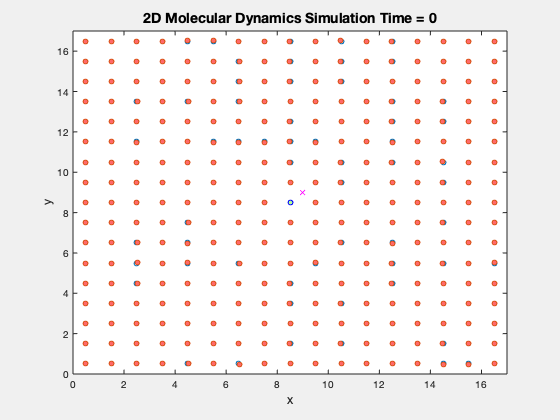
\includegraphics[width=0.50\textwidth]{position_n_289_t_0.png}
    \caption{\small FIG 2: Initial molecule positions}
\end{center}

\begin{center}
    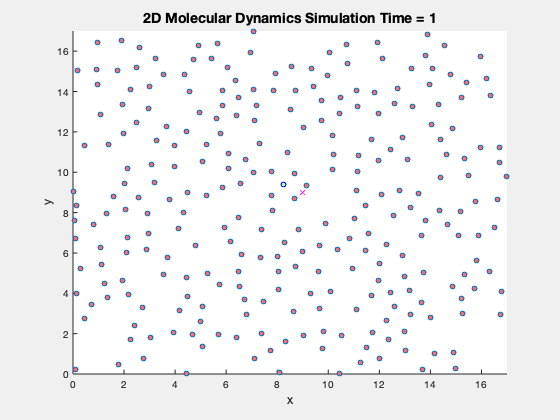
\includegraphics[width=0.50\textwidth]{position_n_289_t_1.png}
    \caption{\small FIG 3: Molecule positions after $t = 1$.}
\end{center}

\begin{center}
    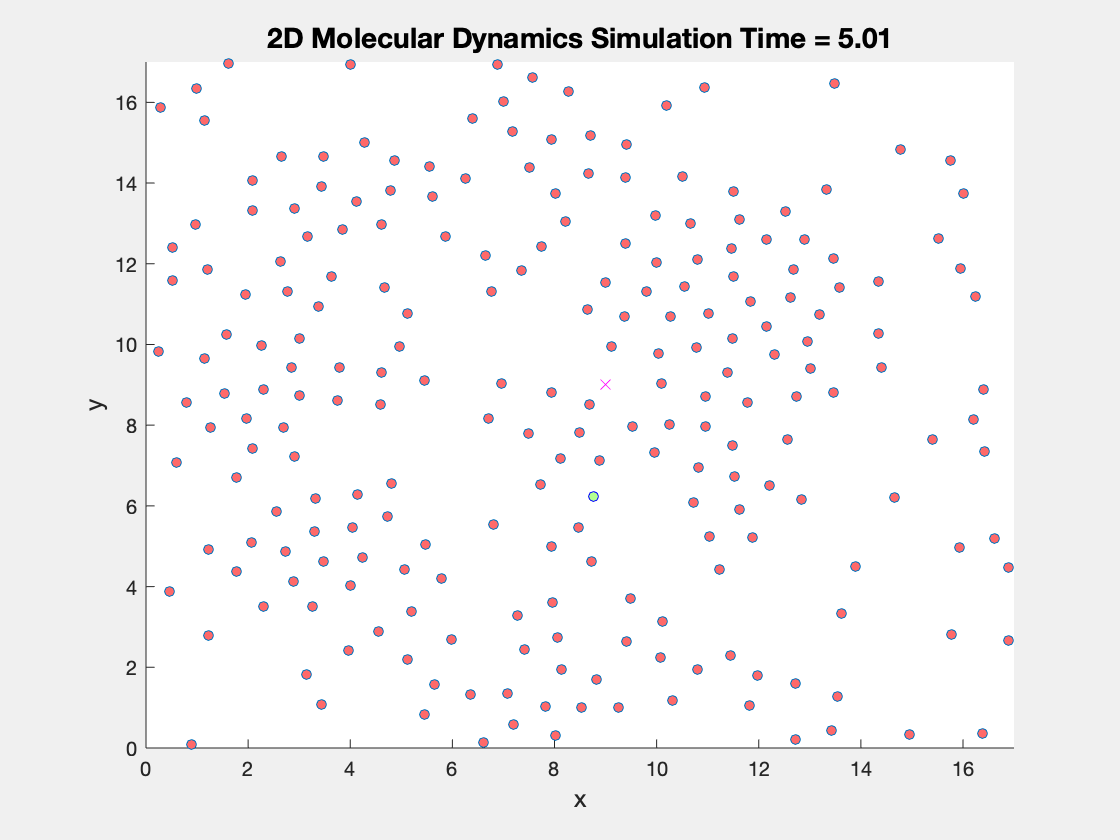
\includegraphics[width=0.50\textwidth]{position_n_289_t_5.01.png}
    \caption{\small FIG 4: Molecule positions after $t = 5$.}
\end{center}

A significant way to test the system is to check if the positions of the molecules are being updated correctly. Running the simulation with the following; $\sigma = 1.5$, $\epsilon = 0.000001$, $m = 1kg$, $T = 300k$, and $n = 289$. Spacing between each molecule is also important, the spacing for all the simulations will just be a unit less $1$. This simulation was also ran without any boundary conditions. \\

This run generates Figure 2, 3, and 4 above, each figure shows the same simulation run at different times. Figure 3 shows how the initial molecules are set up without any force interaction and with $v = 0$. In this figure a small magenta x marks the center of the initial set up box. Near this x, a green molecule is placed near it on the start up. Figure 3 is generated when time $t = 1$, which shows that the molecular interactions are forcing some of the molecules out of the $n \times n box$. However, the green molecule is not shown to move far from the magenta x. In fact the distance from the x to the green molecule is about the same distance as they were in Figure 2. Starting with $289$ molecules, it is clear from this image that there are less molecules than what was in Figure 3. \\

The molecules with initial conditions around the boundary are first attracted in before having no restrictions to move to infinity in all directions. Therefore, these molecules will continuously move away from the center of the box having no forces from the other molecules to bring them back in. As long as there is no outside forces these molecules will continue to move  away forever. Finally, Figure 4 shows that even more molecules have left the original $n \times n$ box. The molecules also seem to have formed different cluster regions. The green molecule now is even further from the center of the box and has less molecules surrounding it, meaning that all molecules that are now spread out like this will have more freedom to move around with less interactions. As time continues and the time step becomes very large, it is possible that there will be no remaining molecules in the original $18 \times 18$ box. \\

Furthermore, this prior was ran with the Verlet integration method. Running the simulation with the same initial conditions except using the Euler integration method will produce the same results. Now, changing the simulation to have boundary conditions will change the results discovered in the previous figures. Using the same initial conditions as before with the Verlet integration method produces the following figure below.

\begin{center}
    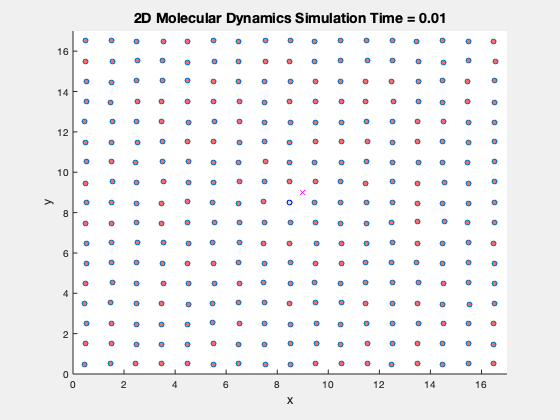
\includegraphics[width=0.50\textwidth]{position_n_289_t_0.01_bc.png}
    \caption{\small FIG 2: Initial molecule positions Molecule positions from Verlet integration numerical method.}
\end{center}

At time $t = 0.01$, nothing about this result changes from the following run. This should be expected since this is just setting up the positions and no forces should overpower each molecule. Allowing time to continue in the simulation produces the next Figure. 

\begin{center}
    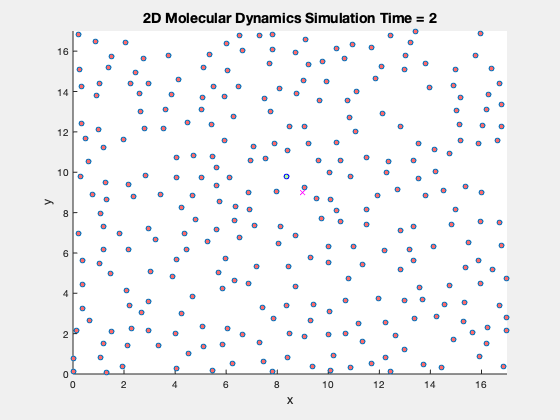
\includegraphics[width=0.50\textwidth]{position_n_289_t_2_bc.png}
    \caption{\small FIG 3: Molecule positions from Verlet integration numerical method after $t = 1$.}
\end{center}

The snapshot of this figure was taken at time $t = 2$. The initial green molecule that starts in the center of the box is still around the center of the box. Since the molecules can not leave the box boundaries, all of the initial molecules are still accounted for. A tighter packed area with the spacing between each molecule reduced will actually make the molecules stay in place, the molecules will end up just jiggling around in their fixed position much like a solid. Many of the molecules are close to their initial starting positions even though a lot more time has gone by. The way the boundary works is that when the molecule hits the wall, the molecule bounces off of the wall with the same velocity. 

\begin{center}
    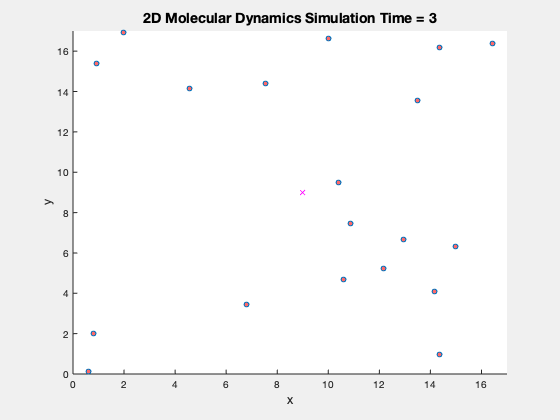
\includegraphics[width=0.50\textwidth]{position_n_289_t_3_bc.png}
    \caption{\small FIG 4: Molecule positions from Verlet integration numerical method after $t = 5$.}
\end{center}

Increasing time one more time shows some unexpected results with the boundary conditions. As seen in Figure there is only a fraction on molecules left in the simulation at time $t = 3$. Prior to this screenshot shows that a few molecules increase in velocity, then rapidly increase in velocity passing by slower moving molecules and bouncing off the walls. This then results in the molecules popping into and out of existence in the box. This is the result in a numerical error caused by the numerical integrator, Verlet. What happens is the step size becomes too large when a particle starts moving to fast. A single particle will cause the whole system to go into chaos because its velocity is too large. It will start cause the calculation of other particles to increase the velocity and eventually lose the particle, the particle will no longer be bounded within the box. However, this error in the integrator takes a while to occur. Running this method with Euler's numerical integrator produces the image below. 

\begin{center}
    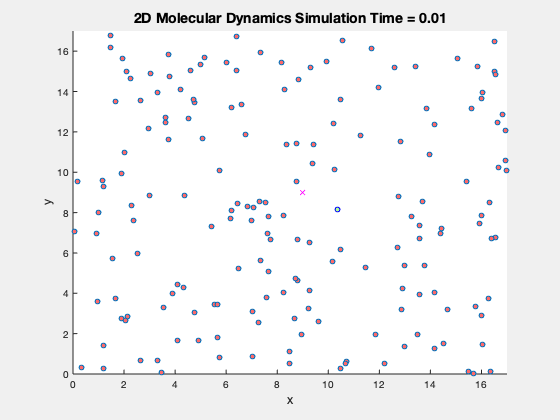
\includegraphics[width=0.50\textwidth]{position_n_289_t_0_bc_euler.png}
    \caption{\small FIG 5: Initial molecule positions from Euler integration numerical method.}
\end{center}

Given the same initial conditions as the Verlet numerical method, at time $t = 0.01$ the system is already chaotic. Instead of the molecules being close to the initial start positions, the molecules are already on a much later time step in comparison to the Verlet method. The molecules in the system for this scenario with these initial conditions are in a space that is too small for what the forces impose on each molecule. In this small space. A molecule that gains too much energy is bound by this space and eventually will excite the other molecules too fast. The speed at which this occurs depends on the given numerical method and time step. In this case, the time step are slow to measure the force better. Eventually, the molecules will break out of these boundary conditions and will disappear from the initial positions, as seen in the figure below. 

\begin{center}
    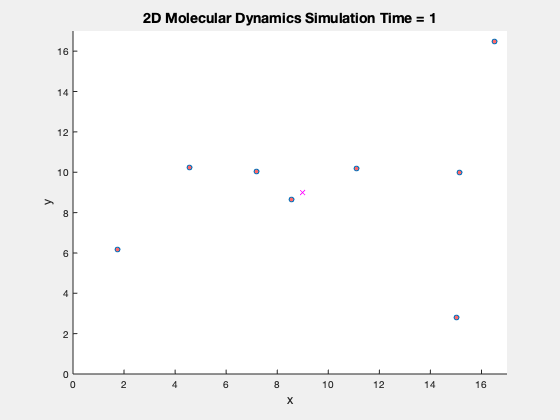
\includegraphics[width=0.50\textwidth]{position_n_289_t_1_bc_euler.png}
    \caption{\small FIG 6: Molecule positions from Euler integration numerical method after $t = 1$.}
\end{center}

At time $t = 1$ the simulation is clearly broke and is far from how the simulation looked when running the Verlet method. Not much time has passed during the Euler's method run, yet in the plot it is easy to count how many molecules remain in the system. The main problem with this isn't to see where and how the molecules are moving, however, in this instance it is visually clear to see that this is failing. From this we know not to take any data from it. The main idea of this simulation is to get energy values out of the simulation. This is what the Lennard-Jones potential is based on, it is only a result of equation (1) that we get these visualizations. It then reassures us that the molecules in the system are behaving correctly and that the energy values are accurate. Therefore, when running this simulation, specific initial conditions mused be pick so that there are no wrong energy calculations. \\

There are many ways to fix this problem, one of the first and easiest ways is to increase the spacing between each molecule. This will make it so that the system is not compressed and will allow more room for molecules to move passed each other. In return, there will be less interactions and less force. In setting the initial conditions to this, it delays the chaotic velocity we will see from the boundary conditions.\\

Changing some of the initial conditions will change how well the simulation will run. Changing the value of $\epsilon$ to something much larger, $\epsilon = 100$, will increase both forces. The system will attract all of the molecules to the center of the box. The the repulsive force will take over sending the system into a chaotic state. This repulsive force is similar to that of an implosion and then a sudden explosion of molecules.  If $\epsilon$ is made very small on the order of $10^{-15}$, then the forces that are calculated are minuscule. The calculated forces will be so small that it would appear that there is no attractive or repulsive force between any molecule.  \\

The other significant variable is $\sigma$. First, if $\sigma$ is very small, on the order of $10^{-15}$, then the repulsive force becomes very weak. Although the force is very weak it is still evident in the simulation. The molecules will come very close to each other to the point of touching, but they will never pass through each other. On the other extreme, if $\sigma$ is made slightly larger than the initial value, the repulsive function becomes very strong. At $\sigma = 7$ the molecules immediately start to rapidly move away from each other at $t = 0.01$. Any value of $\sigma > 7$ while $\epsilon = 10^{5}$ is unstable. \\

Knowing what all the inputs should be to run a stable simulation, data can now be extracted from the simulation. Below shows a figure of the total energy of the system using the very first initial conditions. 

\begin{center}
    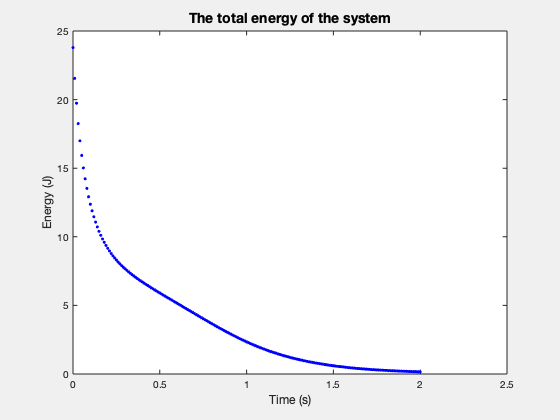
\includegraphics[width=0.50\textwidth]{energy_t_2.png}
    \caption{\small FIG 7: Total energy of the system using the initial conditions up to $t = 2$.}
\end{center}



\subsection{Molecular Dynamics 3D System Discussion}

Finally, this simulation can be scaled up to 3 dimensions. In 3 dimensions, this allows for the molecules to have an extra degree of freedom, which can result in very different outcomes given the same input as the 2 dimensional case. An increase in dimensions also means that there will be an increase in computation time and effort. The simulation will now have to keep trace of a third coordinate and everything that is attached to this coordinate such as force, acceleration, and position. The following figure is an example from the 3D simulation program. Since the world around us is 3 dimensions, the simulations ran should generally be in 3 dimensions. While not always true, a simulation in 3D can give a more accurate description of how the system is behaving. This extra coordinate also can run simulations in geometries that are not found in 2 dimensions. Given real world applications, this simulation would better tell an outcome. 

\begin{center}
    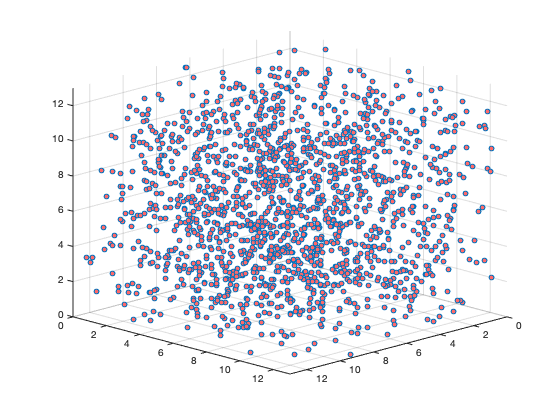
\includegraphics[width=0.50\textwidth]{3d.png}
    \caption{\small FIG 8: 3D example of the molecular dynamics simulation.}
\end{center}

The figure above demos a simple simulation to the 3D after some time. The demo above took longer to run than the 2D simulation. Due to an increase in molecules and an increase in the amount of calculations needed. 3D plots are typically harder to read and not as useful. Running a simulation like this can tell us a lot about the total energy of a system and give a more accurate result to a real world experiment. 

\section{\label{sec:level4} CONCLUSION} 

Molecular dynamic simulations are complex and many different scenarios and parameters can be changed in a given experiment. The Lennard-Jones potential is a great equation to build a simple model. From the Lennard-Jones potential there are two main forces to investigate, the attraction force and the repulsive force. \\

There are different phases of a material that can be modeled, solid, liquid, and gas. Useful simulations will try and find out what is happening at edge cases, that is, simulations that are ran from phase transformations and the critical point of a material. While different phases can be modeled, it is easiest to model a gas at room temperature. \\

Understanding the simulations parameters, a stable experiment can be ran. From he experiment a few pieces of information can be pulled out. The total energy, kinetic energy, and the potential energy of the system will tell if the energy was conserved. 


\section{\label{sec:level3}FUTURE WORK} 

Molecular Dynamics is a study in which a lot of different levers can be pulled to get different results. This simulation represents molecular dynamics in its most basic form, that is, this is one of the most basic simulation one can create to model a system on particles. This simulation is important within it's building blocks. There are many modifications that can be made to this program to get different results. It could be that the end results are to figure out a faster way to run a complex simulation, then different computational methods as well as different numerical techniques could be implemented. As previously discussed, there are different phases a material could be observed. Such as a solid, liquid, or gas. This simulation would also be good to find the results of a material at its critical point or at the transitioning phases.


\section{\label{sec:level3}CITATIONS AND REFERENCES}

[1]  H. Aktulga, J. Fogarty, S. Pandit, and A. Grama, “Parallel reactive molecular dynamics:Numerical methods and algorithmic techniques,”Parallel Computing,  vol. 38,  no. 4,  pp.245  –  259,  2012.  [Online].  \\

\\

[2]  M. Griebel, S. Knapek, and G. Zumbusch,Numerical Simulation in Molecular Dynamics:Numerics, Algorithms, Parallelization, Applications, 1st ed.  Springer Publishing Company,Incorporated, 2010. \\

\\

[3]  B. Leimkuhler and C. Matthews,Molecular Dynamics: With Deterministic and StochasticNumerical Methods, ser. Interdisciplinary Applied Mathematics.    Springer, May 2015. \\

\\

[4]  Y.-W. Li and M. P. Ciamarra, “Phase behaviour of lennard-jones particles in two dimen-sions,” 2020. \\

\\

[5]  D. Lu, H. Wang, M. Chen, J. Liu, L. Lin, R. Car, W. E, W. Jia, and L. Zhang, “86 pflopsdeep potential molecular dynamics simulation of 100 million atoms with ab initio accuracy,”2020. \\

\end{multicols}

%\clearpage
%\onecolumn



\clearpage
\onecolumngrid
\appendix

\section*{Appendix} 
\subsection{Molecular Dynamics 2D Program}
\lstinputlisting{md_2d_sim.m}

\subsection{Molecular Dynamics 3D Program}
\lstinputlisting{md_3d_sim.m}

\end{document}